\documentclass[twoside]{book}

% Packages required by doxygen
\usepackage{fixltx2e}
\usepackage{calc}
\usepackage{doxygen}
\usepackage[export]{adjustbox} % also loads graphicx
\usepackage{graphicx}
\usepackage[utf8]{inputenc}
\usepackage{makeidx}
\usepackage{multicol}
\usepackage{multirow}
\PassOptionsToPackage{warn}{textcomp}
\usepackage{textcomp}
\usepackage[nointegrals]{wasysym}
\usepackage[table]{xcolor}

% Font selection
\usepackage[T1]{fontenc}
\usepackage[scaled=.90]{helvet}
\usepackage{courier}
\usepackage{amssymb}
\usepackage{sectsty}
\renewcommand{\familydefault}{\sfdefault}
\allsectionsfont{%
  \fontseries{bc}\selectfont%
  \color{darkgray}%
}
\renewcommand{\DoxyLabelFont}{%
  \fontseries{bc}\selectfont%
  \color{darkgray}%
}
\newcommand{\+}{\discretionary{\mbox{\scriptsize$\hookleftarrow$}}{}{}}

% Page & text layout
\usepackage{geometry}
\geometry{%
  a4paper,%
  top=2.5cm,%
  bottom=2.5cm,%
  left=2.5cm,%
  right=2.5cm%
}
\tolerance=750
\hfuzz=15pt
\hbadness=750
\setlength{\emergencystretch}{15pt}
\setlength{\parindent}{0cm}
\setlength{\parskip}{3ex plus 2ex minus 2ex}
\makeatletter
\renewcommand{\paragraph}{%
  \@startsection{paragraph}{4}{0ex}{-1.0ex}{1.0ex}{%
    \normalfont\normalsize\bfseries\SS@parafont%
  }%
}
\renewcommand{\subparagraph}{%
  \@startsection{subparagraph}{5}{0ex}{-1.0ex}{1.0ex}{%
    \normalfont\normalsize\bfseries\SS@subparafont%
  }%
}
\makeatother

% Headers & footers
\usepackage{fancyhdr}
\pagestyle{fancyplain}
\fancyhead[LE]{\fancyplain{}{\bfseries\thepage}}
\fancyhead[CE]{\fancyplain{}{}}
\fancyhead[RE]{\fancyplain{}{\bfseries\leftmark}}
\fancyhead[LO]{\fancyplain{}{\bfseries\rightmark}}
\fancyhead[CO]{\fancyplain{}{}}
\fancyhead[RO]{\fancyplain{}{\bfseries\thepage}}
\fancyfoot[LE]{\fancyplain{}{}}
\fancyfoot[CE]{\fancyplain{}{}}
\fancyfoot[RE]{\fancyplain{}{\bfseries\scriptsize Generated by Doxygen }}
\fancyfoot[LO]{\fancyplain{}{\bfseries\scriptsize Generated by Doxygen }}
\fancyfoot[CO]{\fancyplain{}{}}
\fancyfoot[RO]{\fancyplain{}{}}
\renewcommand{\footrulewidth}{0.4pt}
\renewcommand{\chaptermark}[1]{%
  \markboth{#1}{}%
}
\renewcommand{\sectionmark}[1]{%
  \markright{\thesection\ #1}%
}

% Indices & bibliography
\usepackage{natbib}
\usepackage[titles]{tocloft}
\setcounter{tocdepth}{3}
\setcounter{secnumdepth}{5}
\makeindex

% Hyperlinks (required, but should be loaded last)
\usepackage{ifpdf}
\ifpdf
  \usepackage[pdftex,pagebackref=true]{hyperref}
\else
  \usepackage[ps2pdf,pagebackref=true]{hyperref}
\fi
\hypersetup{%
  colorlinks=true,%
  linkcolor=blue,%
  citecolor=blue,%
  unicode%
}

% Custom commands
\newcommand{\clearemptydoublepage}{%
  \newpage{\pagestyle{empty}\cleardoublepage}%
}

\usepackage{caption}
\captionsetup{labelsep=space,justification=centering,font={bf},singlelinecheck=off,skip=4pt,position=top}

%===== C O N T E N T S =====

\begin{document}

% Titlepage & ToC
\hypersetup{pageanchor=false,
             bookmarksnumbered=true,
             pdfencoding=unicode
            }
\pagenumbering{alph}
\begin{titlepage}
\vspace*{7cm}
\begin{center}%
{\Large My Project }\\
\vspace*{1cm}
{\large Generated by Doxygen 1.8.13}\\
\end{center}
\end{titlepage}
\clearemptydoublepage
\pagenumbering{roman}
\tableofcontents
\clearemptydoublepage
\pagenumbering{arabic}
\hypersetup{pageanchor=true}

%--- Begin generated contents ---
\chapter{Todo-\/\+List}
\label{md_Todo}
\Hypertarget{md_Todo}
\subsection*{General}


\begin{DoxyItemize}
\item Font object should be inside a extra class, i.\+e. font\+Object inside \hyperlink{Game_8h}{Game.\+h} --$>$ im moment hat jedes Modul die gleiche Font Objekte im Speicher und auch die Logig diese zu erstellen
\item Problem mit iterieren über drawable vectoren --$>$ allg. lösung dafür finden!
\item center all the stuff inside rects based on their bounds!
\item die ganzen handle event sachen in ein switch case packen, wird übersichtlicher
\item Mouse pos stuff in toolbox auslagern
\end{DoxyItemize}

\subsection*{\hyperlink{classMainMenu}{Main\+Menu}}


\begin{DoxyItemize}
\item Name eingeben und möglichen übergang zur Lobbyübersicht implementieren!
\item Doc weiterschreiben \subsection*{\hyperlink{classGameView}{Game\+View}}
\end{DoxyItemize}


\begin{DoxyItemize}
\item evtl eine andere Textur für die void Felder, eine etwas dunklere wäre da cooler
\item Menu nicht nur game verlassen, sondern dialog implementieren, wo eine möglichkeit spiel verlassen ist
\item Format score
\item Doc weiter schreiben
\end{DoxyItemize}

\subsection*{change\+Name\+Menu}


\begin{DoxyItemize}
\item write entered name to file --$>$ enter funktioniert so erstmal noch nicht 
\end{DoxyItemize}
\chapter{Module Index}
\section{Modules}
Here is a list of all modules\+:\begin{DoxyCompactList}
\item \contentsline{section}{General Purpose}{\pageref{group__genPurpose}}{}
\item \contentsline{section}{Game View}{\pageref{group__gameView}}{}
\item \contentsline{section}{Main Menu}{\pageref{group__MainMenu}}{}
\end{DoxyCompactList}

\chapter{Class Index}
\section{Class List}
Here are the classes, structs, unions and interfaces with brief descriptions\+:\begin{DoxyCompactList}
\item\contentsline{section}{\hyperlink{classMainMenu}{Main\+Menu} \\*\hyperlink{classMainMenu}{Main\+Menu} functionality is implemented in here }{\pageref{classMainMenu}}{}
\end{DoxyCompactList}

\chapter{File Index}
\section{File List}
Here is a list of all documented files with brief descriptions\+:\begin{DoxyCompactList}
\item\contentsline{section}{\hyperlink{MainMenu_8cpp}{Main\+Menu.\+cpp} }{\pageref{MainMenu_8cpp}}{}
\item\contentsline{section}{\hyperlink{MainMenu_8h}{Main\+Menu.\+h} \\*Defining \hyperlink{classMainMenu}{Main\+Menu} }{\pageref{MainMenu_8h}}{}
\end{DoxyCompactList}

\chapter{Module Documentation}
\hypertarget{group__genPurpose}{}\section{General Purpose}
\label{group__genPurpose}\index{General Purpose@{General Purpose}}


in this header some general purpose things, helper functions and game state are implemented  


in this header some general purpose things, helper functions and game state are implemented 

in this header some general purpose things, helper functions and game state are defined

\begin{DoxyAuthor}{Author}
Marco Deuscher 
\end{DoxyAuthor}
\begin{DoxyDate}{Date}
10.\+11.\+2019
\end{DoxyDate}
\begin{DoxyAuthor}{Author}
Marco Deuscher 
\end{DoxyAuthor}
\begin{DoxyDate}{Date}
07.\+11.\+2019 
\end{DoxyDate}

\hypertarget{group__gameView}{}\section{Game View}
\label{group__gameView}\index{Game View@{Game View}}


All the game logic and display are inside this class.  


All the game logic and display are inside this class. 

\begin{DoxyAuthor}{Author}
Marco Deuscher 
\end{DoxyAuthor}
\begin{DoxyDate}{Date}
07.\+11.\+2019 
\end{DoxyDate}

\hypertarget{group__MainMenu}{}\section{Main Menu}
\label{group__MainMenu}\index{Main Menu@{Main Menu}}


Implementing Main Menu.  


\subsection*{Files}
\begin{DoxyCompactItemize}
\item 
file \hyperlink{MainMenu_8h}{Main\+Menu.\+h}
\begin{DoxyCompactList}\small\item\em defining \hyperlink{classMainMenu}{Main\+Menu} \end{DoxyCompactList}\end{DoxyCompactItemize}


\subsection{Detailed Description}
Implementing Main Menu. 

\begin{DoxyAuthor}{Author}
Marco Deuscher 
\end{DoxyAuthor}
\begin{DoxyDate}{Date}
05.\+11.\+2019 
\end{DoxyDate}

\chapter{Class Documentation}
\hypertarget{classChangeNameMenu}{}\section{Change\+Name\+Menu Class Reference}
\label{classChangeNameMenu}\index{Change\+Name\+Menu@{Change\+Name\+Menu}}
\subsection*{Public Member Functions}
\begin{DoxyCompactItemize}
\item 
\mbox{\Hypertarget{classChangeNameMenu_aee87255f196fefc48b22cd3ac8dc5dd2}\label{classChangeNameMenu_aee87255f196fefc48b22cd3ac8dc5dd2}} 
{\bfseries Change\+Name\+Menu} (sf\+::\+Render\+Window $\ast$window, const int window\+Width, const int window\+Height, game\+State $\ast$gs)
\item 
\mbox{\Hypertarget{classChangeNameMenu_af0e30625ee17bebc5c6792732913af3f}\label{classChangeNameMenu_af0e30625ee17bebc5c6792732913af3f}} 
int {\bfseries init\+Change\+Name\+Menu} ()
\item 
\mbox{\Hypertarget{classChangeNameMenu_a6e2b6699d594b54b1d6f0e0680cfaa16}\label{classChangeNameMenu_a6e2b6699d594b54b1d6f0e0680cfaa16}} 
void {\bfseries handle\+Change\+Name\+Menu} ()
\end{DoxyCompactItemize}


The documentation for this class was generated from the following files\+:\begin{DoxyCompactItemize}
\item 
Change\+Name\+Menu.\+h\item 
Change\+Name\+Menu.\+cpp\end{DoxyCompactItemize}

\hypertarget{classGameView}{}\section{Game\+View Class Reference}
\label{classGameView}\index{Game\+View@{Game\+View}}
\subsection*{Public Member Functions}
\begin{DoxyCompactItemize}
\item 
\hyperlink{classGameView_a41cabebb48225d25835052e275fa0bce}{Game\+View} (sf\+::\+Render\+Window $\ast$game\+Window, const int windoow\+Width, const int window\+Height, game\+State $\ast$gs)
\item 
int \hyperlink{classGameView_affc208b835faeede0f435197e1440951}{init\+Game\+View} ()
\item 
\mbox{\Hypertarget{classGameView_a8a93e2963678fc897a231b4b6dae2ee2}\label{classGameView_a8a93e2963678fc897a231b4b6dae2ee2}} 
int {\bfseries handle\+Game\+View} ()
\item 
\mbox{\Hypertarget{classGameView_aa1bbff949a105e458f2dbf6c6cc3b9be}\label{classGameView_aa1bbff949a105e458f2dbf6c6cc3b9be}} 
void {\bfseries set\+Score} (int score\+Red, int score\+Blue)
\item 
\mbox{\Hypertarget{classGameView_ad7b959dc103564bdfbc869379386b4c5}\label{classGameView_ad7b959dc103564bdfbc869379386b4c5}} 
void {\bfseries set\+Move\+Tracker} (bool red)
\end{DoxyCompactItemize}


\subsection{Constructor \& Destructor Documentation}
\mbox{\Hypertarget{classGameView_a41cabebb48225d25835052e275fa0bce}\label{classGameView_a41cabebb48225d25835052e275fa0bce}} 
\index{Game\+View@{Game\+View}!Game\+View@{Game\+View}}
\index{Game\+View@{Game\+View}!Game\+View@{Game\+View}}
\subsubsection{\texorpdfstring{Game\+View()}{GameView()}}
{\footnotesize\ttfamily Game\+View\+::\+Game\+View (\begin{DoxyParamCaption}\item[{sf\+::\+Render\+Window $\ast$}]{gw,  }\item[{const int}]{window\+Width,  }\item[{const int}]{window\+Height,  }\item[{game\+State $\ast$}]{gs }\end{DoxyParamCaption})}


\begin{DoxyParams}{Parameters}
{\em game\+Window} & \\
\hline
{\em window\+Width} & \\
\hline
{\em window\+Height} & \\
\hline
{\em gs} & \\
\hline
\end{DoxyParams}


\subsection{Member Function Documentation}
\mbox{\Hypertarget{classGameView_affc208b835faeede0f435197e1440951}\label{classGameView_affc208b835faeede0f435197e1440951}} 
\index{Game\+View@{Game\+View}!init\+Game\+View@{init\+Game\+View}}
\index{init\+Game\+View@{init\+Game\+View}!Game\+View@{Game\+View}}
\subsubsection{\texorpdfstring{init\+Game\+View()}{initGameView()}}
{\footnotesize\ttfamily int Game\+View\+::init\+Game\+View (\begin{DoxyParamCaption}{ }\end{DoxyParamCaption})}

\begin{DoxyReturn}{Returns}

\end{DoxyReturn}


The documentation for this class was generated from the following files\+:\begin{DoxyCompactItemize}
\item 
Game\+View.\+h\item 
Game\+View.\+cpp\end{DoxyCompactItemize}

\hypertarget{classMainMenu}{}\section{Main\+Menu Class Reference}
\label{classMainMenu}\index{Main\+Menu@{Main\+Menu}}


\hyperlink{classMainMenu}{Main\+Menu} functionality is implemented in here.  




{\ttfamily \#include $<$Main\+Menu.\+h$>$}

\subsection*{Public Member Functions}
\begin{DoxyCompactItemize}
\item 
\hyperlink{classMainMenu_a7d77dec9912147828eafc561a908ffed}{Main\+Menu} (sf\+::\+Render\+Window $\ast$window, const int window\+Width, const int window\+Height, game\+State $\ast$gs)
\begin{DoxyCompactList}\small\item\em Constructor. \end{DoxyCompactList}\item 
int \hyperlink{classMainMenu_a3c15af2faff50d642ab6920e2fdcd297}{init\+Main\+Menu} ()
\begin{DoxyCompactList}\small\item\em initializing \hyperlink{classMainMenu}{Main\+Menu} \end{DoxyCompactList}\item 
int \hyperlink{classMainMenu_ab849dbe0f56adfed51f58e80a536c5f8}{handle\+Main\+Menu} ()
\begin{DoxyCompactList}\small\item\em this function is called from the main game loop \end{DoxyCompactList}\end{DoxyCompactItemize}


\subsection{Detailed Description}
\hyperlink{classMainMenu}{Main\+Menu} functionality is implemented in here. 

\subsection{Constructor \& Destructor Documentation}
\mbox{\Hypertarget{classMainMenu_a7d77dec9912147828eafc561a908ffed}\label{classMainMenu_a7d77dec9912147828eafc561a908ffed}} 
\index{Main\+Menu@{Main\+Menu}!Main\+Menu@{Main\+Menu}}
\index{Main\+Menu@{Main\+Menu}!Main\+Menu@{Main\+Menu}}
\subsubsection{\texorpdfstring{Main\+Menu()}{MainMenu()}}
{\footnotesize\ttfamily Main\+Menu\+::\+Main\+Menu (\begin{DoxyParamCaption}\item[{sf\+::\+Render\+Window $\ast$}]{window,  }\item[{const int}]{window\+Width,  }\item[{const int}]{window\+Height,  }\item[{game\+State $\ast$}]{gs }\end{DoxyParamCaption})}



Constructor. 


\begin{DoxyParams}{Parameters}
{\em window} & Window in which the main menu is drawn \\
\hline
{\em window\+Width} & width of the given window \\
\hline
{\em window\+Height} & height of the given window \\
\hline
\end{DoxyParams}


\subsection{Member Function Documentation}
\mbox{\Hypertarget{classMainMenu_ab849dbe0f56adfed51f58e80a536c5f8}\label{classMainMenu_ab849dbe0f56adfed51f58e80a536c5f8}} 
\index{Main\+Menu@{Main\+Menu}!handle\+Main\+Menu@{handle\+Main\+Menu}}
\index{handle\+Main\+Menu@{handle\+Main\+Menu}!Main\+Menu@{Main\+Menu}}
\subsubsection{\texorpdfstring{handle\+Main\+Menu()}{handleMainMenu()}}
{\footnotesize\ttfamily int Main\+Menu\+::handle\+Main\+Menu (\begin{DoxyParamCaption}{ }\end{DoxyParamCaption})}



this function is called from the main game loop 

in this function the sprites/text etc. are drawn, this function is called from the main thread

\begin{DoxyReturn}{Returns}
M\+A\+I\+N\+M\+E\+N\+U\+\_\+\+S\+U\+C\+C\+E\+SS if successfull 
\end{DoxyReturn}
\mbox{\Hypertarget{classMainMenu_a3c15af2faff50d642ab6920e2fdcd297}\label{classMainMenu_a3c15af2faff50d642ab6920e2fdcd297}} 
\index{Main\+Menu@{Main\+Menu}!init\+Main\+Menu@{init\+Main\+Menu}}
\index{init\+Main\+Menu@{init\+Main\+Menu}!Main\+Menu@{Main\+Menu}}
\subsubsection{\texorpdfstring{init\+Main\+Menu()}{initMainMenu()}}
{\footnotesize\ttfamily int Main\+Menu\+::init\+Main\+Menu (\begin{DoxyParamCaption}{ }\end{DoxyParamCaption})}



initializing \hyperlink{classMainMenu}{Main\+Menu} 

in this function all the objects are created, font loaded etc.

\begin{DoxyNote}{Note}
in this init function the font is loaded, the text initialized
\end{DoxyNote}
\begin{DoxyReturn}{Returns}
M\+A\+I\+N\+M\+E\+N\+U\+\_\+\+F\+O\+N\+T\+L\+O\+A\+D\+I\+N\+G\+\_\+\+E\+R\+R\+OR if loading the font failed, M\+A\+I\+N\+M\+E\+N\+U\+\_\+\+S\+U\+C\+C\+E\+SS if successfull 
\end{DoxyReturn}


The documentation for this class was generated from the following files\+:\begin{DoxyCompactItemize}
\item 
\hyperlink{MainMenu_8h}{Main\+Menu.\+h}\item 
\hyperlink{MainMenu_8cpp}{Main\+Menu.\+cpp}\end{DoxyCompactItemize}

\chapter{File Documentation}
\hypertarget{Game_8cpp}{}\section{Game.\+cpp File Reference}
\label{Game_8cpp}\index{Game.\+cpp@{Game.\+cpp}}
{\ttfamily \#include $<$fstream$>$}\newline
{\ttfamily \#include $<$sstream$>$}\newline
{\ttfamily \#include \char`\"{}Game.\+h\char`\"{}}\newline
Include dependency graph for Game.\+cpp\+:\nopagebreak
\begin{figure}[H]
\begin{center}
\leavevmode
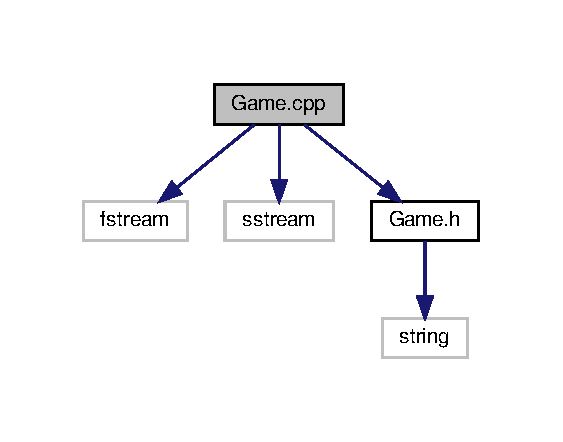
\includegraphics[width=270pt]{Game_8cpp__incl}
\end{center}
\end{figure}
\subsection*{Functions}
\begin{DoxyCompactItemize}
\item 
std\+::string \hyperlink{Game_8cpp_aa3736356897a975aa36b5bbfdbba22a3}{get\+String\+From\+File} (std\+::string filepath)
\begin{DoxyCompactList}\small\item\em reads a String form the specified file into a buffer and returns a std\+::string Object, can be used to get text ressources for i.\+e. buttons, textfields etc. \end{DoxyCompactList}\end{DoxyCompactItemize}


\subsection{Function Documentation}
\mbox{\Hypertarget{Game_8cpp_aa3736356897a975aa36b5bbfdbba22a3}\label{Game_8cpp_aa3736356897a975aa36b5bbfdbba22a3}} 
\index{Game.\+cpp@{Game.\+cpp}!get\+String\+From\+File@{get\+String\+From\+File}}
\index{get\+String\+From\+File@{get\+String\+From\+File}!Game.\+cpp@{Game.\+cpp}}
\subsubsection{\texorpdfstring{get\+String\+From\+File()}{getStringFromFile()}}
{\footnotesize\ttfamily std\+::string get\+String\+From\+File (\begin{DoxyParamCaption}\item[{std\+::string}]{filepath }\end{DoxyParamCaption})}



reads a String form the specified file into a buffer and returns a std\+::string Object, can be used to get text ressources for i.\+e. buttons, textfields etc. 


\begin{DoxyParams}{Parameters}
{\em filepath} & specifies path to text file that is supposed to be read \\
\hline
\end{DoxyParams}
\begin{DoxyReturn}{Returns}
String read in String 
\end{DoxyReturn}

\hypertarget{Game_8h}{}\section{Game.\+h File Reference}
\label{Game_8h}\index{Game.\+h@{Game.\+h}}
{\ttfamily \#include $<$string$>$}\newline
Include dependency graph for Game.\+h\+:\nopagebreak
\begin{figure}[H]
\begin{center}
\leavevmode
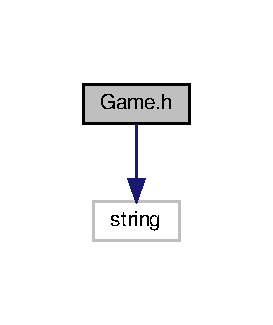
\includegraphics[width=131pt]{Game_8h__incl}
\end{center}
\end{figure}
This graph shows which files directly or indirectly include this file\+:\nopagebreak
\begin{figure}[H]
\begin{center}
\leavevmode
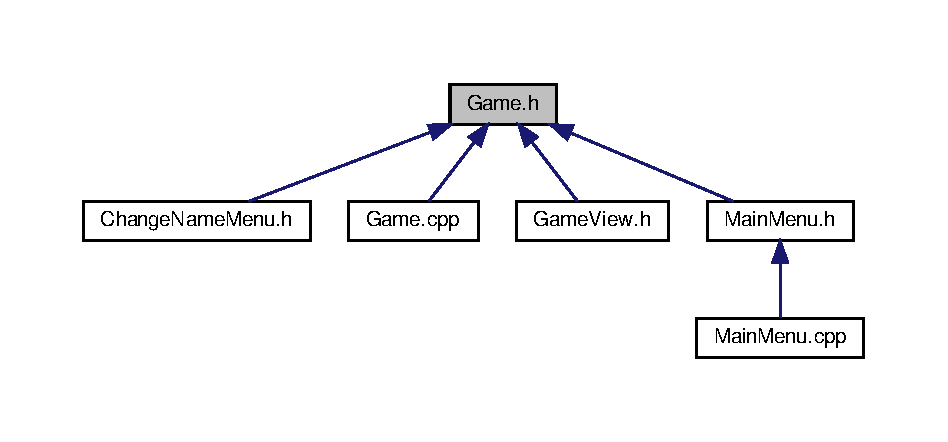
\includegraphics[width=350pt]{Game_8h__dep__incl}
\end{center}
\end{figure}
\subsection*{Enumerations}
\begin{DoxyCompactItemize}
\item 
\mbox{\Hypertarget{Game_8h_aaf29bbe309504beb4cfec2481eacee62}\label{Game_8h_aaf29bbe309504beb4cfec2481eacee62}} 
enum {\bfseries game\+State} \{ {\bfseries M\+A\+I\+N\+M\+E\+NU}, 
{\bfseries I\+N\+G\+A\+ME}, 
{\bfseries C\+H\+A\+N\+G\+E\+N\+A\+ME}
 \}
\end{DoxyCompactItemize}
\subsection*{Functions}
\begin{DoxyCompactItemize}
\item 
std\+::string \hyperlink{Game_8h_aa3736356897a975aa36b5bbfdbba22a3}{get\+String\+From\+File} (std\+::string filepath)
\begin{DoxyCompactList}\small\item\em reads a String form the specified file into a buffer and returns a std\+::string Object, can be used to get text ressources for i.\+e. buttons, textfields etc. \end{DoxyCompactList}\end{DoxyCompactItemize}


\subsection{Function Documentation}
\mbox{\Hypertarget{Game_8h_aa3736356897a975aa36b5bbfdbba22a3}\label{Game_8h_aa3736356897a975aa36b5bbfdbba22a3}} 
\index{Game.\+h@{Game.\+h}!get\+String\+From\+File@{get\+String\+From\+File}}
\index{get\+String\+From\+File@{get\+String\+From\+File}!Game.\+h@{Game.\+h}}
\subsubsection{\texorpdfstring{get\+String\+From\+File()}{getStringFromFile()}}
{\footnotesize\ttfamily std\+::string get\+String\+From\+File (\begin{DoxyParamCaption}\item[{std\+::string}]{filepath }\end{DoxyParamCaption})}



reads a String form the specified file into a buffer and returns a std\+::string Object, can be used to get text ressources for i.\+e. buttons, textfields etc. 

read String from File to a String. Can be used for text Ressources


\begin{DoxyParams}{Parameters}
{\em filepath} & specifies path to text file that is supposed to be read \\
\hline
\end{DoxyParams}
\begin{DoxyReturn}{Returns}
String read in String 
\end{DoxyReturn}

\hypertarget{MainMenu_8cpp}{}\section{Main\+Menu.\+cpp File Reference}
\label{MainMenu_8cpp}\index{Main\+Menu.\+cpp@{Main\+Menu.\+cpp}}
{\ttfamily \#include \char`\"{}Main\+Menu.\+h\char`\"{}}\newline
Include dependency graph for Main\+Menu.\+cpp\+:

\hypertarget{MainMenu_8h}{}\section{Main\+Menu.\+h File Reference}
\label{MainMenu_8h}\index{Main\+Menu.\+h@{Main\+Menu.\+h}}


defining \hyperlink{classMainMenu}{Main\+Menu}  


{\ttfamily \#include $<$S\+F\+M\+L/\+Graphics.\+hpp$>$}\newline
Include dependency graph for Main\+Menu.\+h\+:
% FIG 0
This graph shows which files directly or indirectly include this file\+:
% FIG 1
\subsection*{Classes}
\begin{DoxyCompactItemize}
\item 
class \hyperlink{classMainMenu}{Main\+Menu}
\begin{DoxyCompactList}\small\item\em \hyperlink{classMainMenu}{Main\+Menu} functionality is implemented in here. \end{DoxyCompactList}\end{DoxyCompactItemize}
\subsection*{Macros}
\begin{DoxyCompactItemize}
\item 
\mbox{\Hypertarget{MainMenu_8h_a9cbb5cbcf2bc52c6e330ad40f0dec77f}\label{MainMenu_8h_a9cbb5cbcf2bc52c6e330ad40f0dec77f}} 
\#define {\bfseries F\+O\+N\+T\+S\+\_\+\+M\+A\+I\+N\+M\+E\+N\+U\+\_\+\+P\+A\+TH}~(\char`\"{}/home/marco/C\+Lion\+Projects/Cpp\+Proj/S\+F\+ML-\/Game/S\+F\+M\+L\+Test/Fonts/arial.\+ttf\char`\"{})
\item 
\mbox{\Hypertarget{MainMenu_8h_a2425860db201bcdc79163ed02dbf4ccf}\label{MainMenu_8h_a2425860db201bcdc79163ed02dbf4ccf}} 
\#define {\bfseries M\+A\+I\+N\+M\+E\+N\+U\+\_\+\+F\+O\+N\+T\+L\+O\+A\+D\+I\+N\+G\+\_\+\+E\+R\+R\+OR}~((-\/1))
\item 
\mbox{\Hypertarget{MainMenu_8h_a490af5c5af99d7741b133c0858da87b8}\label{MainMenu_8h_a490af5c5af99d7741b133c0858da87b8}} 
\#define {\bfseries M\+A\+I\+N\+M\+E\+N\+U\+\_\+\+S\+U\+C\+C\+E\+SS}~((0))
\end{DoxyCompactItemize}


\subsection{Detailed Description}
defining \hyperlink{classMainMenu}{Main\+Menu} 

\begin{DoxyAuthor}{Author}
Marco Deuscher 
\end{DoxyAuthor}
\begin{DoxyDate}{Date}
05.\+11.\+2019 
\end{DoxyDate}

%--- End generated contents ---

% Index
\backmatter
\newpage
\phantomsection
\clearemptydoublepage
\addcontentsline{toc}{chapter}{Index}
\printindex

\end{document}
